
%% bare_jrnl.tex
%% V1.4b
%% 2015/08/26
%% by Michael Shell
%% see http://www.michaelshell.org/
%% for current contact information.
%%
%% This is a skeleton file demonstrating the use of IEEEtran.cls
%% (requires IEEEtran.cls version 1.8b or later) with an IEEE
%% journal paper.
%%
%% Support sites:
%% http://www.michaelshell.org/tex/ieeetran/
%% http://www.ctan.org/pkg/ieeetran
%% and
%% http://www.ieee.org/

%%*************************************************************************
%% Legal Notice:
%% This code is offered as-is without any warranty either expressed or
%% implied; without even the implied warranty of MERCHANTABILITY or
%% FITNESS FOR A PARTICULAR PURPOSE! 
%% User assumes all risk.
%% In no event shall the IEEE or any contributor to this code be liable for
%% any damages or losses, including, but not limited to, incidental,
%% consequential, or any other damages, resulting from the use or misuse
%% of any information contained here.
%%
%% All comments are the opinions of their respective authors and are not
%% necessarily endorsed by the IEEE.
%%
%% This work is distributed under the LaTeX Project Public License (LPPL)
%% ( http://www.latex-project.org/ ) version 1.3, and may be freely used,
%% distributed and modified. A copy of the LPPL, version 1.3, is included
%% in the base LaTeX documentation of all distributions of LaTeX released
%% 2003/12/01 or later.
%% Retain all contribution notices and credits.
%% ** Modified files should be clearly indicated as such, including  **
%% ** renaming them and changing author support contact information. **
%%*************************************************************************


% *** Authors should verify (and, if needed, correct) their LaTeX system  ***
% *** with the testflow diagnostic prior to trusting their LaTeX platform ***
% *** with production work. The IEEE's font choices and paper sizes can   ***
% *** trigger bugs that do not appear when using other class files.       ***                          ***
% The testflow support page is at:
% http://www.michaelshell.org/tex/testflow/



\documentclass[journal]{hybrid-cloud}
%
% If IEEEtran.cls has not been installed into the LaTeX system files,
% manually specify the path to it like:
% \documentclass[journal]{../sty/IEEEtran}





% Some very useful LaTeX packages include:
% (uncomment the ones you want to load)


% *** MISC UTILITY PACKAGES ***
%
%\usepackage{ifpdf}
% Heiko Oberdiek's ifpdf.sty is very useful if you need conditional
% compilation based on whether the output is pdf or dvi.
% usage:
% \ifpdf
%   % pdf code
% \else
%   % dvi code
% \fi
% The latest version of ifpdf.sty can be obtained from:
% http://www.ctan.org/pkg/ifpdf
% Also, note that IEEEtran.cls V1.7 and later provides a builtin
% \ifCLASSINFOpdf conditional that works the same way.
% When switching from latex to pdflatex and vice-versa, the compiler may
% have to be run twice to clear warning/error messages.






% *** CITATION PACKAGES ***
%
\usepackage{cite}
% cite.sty was written by Donald Arseneau
% V1.6 and later of IEEEtran pre-defines the format of the cite.sty package
% \cite{} output to follow that of the IEEE. Loading the cite package will
% result in citation numbers being automatically sorted and properly
% "compressed/ranged". e.g., [1], [9], [2], [7], [5], [6] without using
% cite.sty will become [1], [2], [5]--[7], [9] using cite.sty. cite.sty's
% \cite will automatically add leading space, if needed. Use cite.sty's
% noadjust option (cite.sty V3.8 and later) if you want to turn this off
% such as if a citation ever needs to be enclosed in parenthesis.
% cite.sty is already installed on most LaTeX systems. Be sure and use
% version 5.0 (2009-03-20) and later if using hyperref.sty.
% The latest version can be obtained at:
% http://www.ctan.org/pkg/cite
% The documentation is contained in the cite.sty file itself.

% ****  Use caption package and its justification option **** 
%
\usepackage[justification=centering]{caption}



% *** GRAPHICS RELATED PACKAGES ***
%
\ifCLASSINFOpdf
  % \usepackage[pdftex]{graphicx}
  % declare the path(s) where your graphic files are
  % \graphicspath{{../pdf/}{../jpeg/}}
  % and their extensions so you won't have to specify these with
  % every instance of \includegraphics
  % \DeclareGraphicsExtensions{.pdf,.jpeg,.png}
\else
  % or other class option (dvipsone, dvipdf, if not using dvips). graphicx
  % will default to the driver specified in the system graphics.cfg if no
  % driver is specified.
  % \usepackage[dvips]{graphicx}
  % declare the path(s) where your graphic files are
  % \graphicspath{{../eps/}}
  % and their extensions so you won't have to specify these with
  % every instance of \includegraphics
  % \DeclareGraphicsExtensions{.eps}
\fi
% graphicx was written by David Carlisle and Sebastian Rahtz. It is
% required if you want graphics, photos, etc. graphicx.sty is already
% installed on most LaTeX systems. The latest version and documentation
% can be obtained at: 
% http://www.ctan.org/pkg/graphicx
% Another good source of documentation is "Using Imported Graphics in
% LaTeX2e" by Keith Reckdahl which can be found at:
% http://www.ctan.org/pkg/epslatex
%
% latex, and pdflatex in dvi mode, support graphics in encapsulated
% postscript (.eps) format. pdflatex in pdf mode supports graphics
% in .pdf, .jpeg, .png and .mps (metapost) formats. Users should ensure
% that all non-photo figures use a vector format (.eps, .pdf, .mps) and
% not a bitmapped formats (.jpeg, .png). The IEEE frowns on bitmapped formats
% which can result in "jaggedy"/blurry rendering of lines and letters as
% well as large increases in file sizes.
%
% You can find documentation about the pdfTeX application at:
% http://www.tug.org/applications/pdftex

\usepackage{graphicx}
\usepackage{refstyle}



% *** MATH PACKAGES ***
%
%\usepackage{amsmath}
% A popular package from the American Mathematical Society that provides
% many useful and powerful commands for dealing with mathematics.
%
% Note that the amsmath package sets \interdisplaylinepenalty to 10000
% thus preventing page breaks from occurring within multiline equations. Use:
%\interdisplaylinepenalty=2500
% after loading amsmath to restore such page breaks as IEEEtran.cls normally
% does. amsmath.sty is already installed on most LaTeX systems. The latest
% version and documentation can be obtained at:
% http://www.ctan.org/pkg/amsmath





% *** SPECIALIZED LIST PACKAGES ***
%
%\usepackage{algorithmic}
% algorithmic.sty was written by Peter Williams and Rogerio Brito.
% This package provides an algorithmic environment fo describing algorithms.
% You can use the algorithmic environment in-text or within a figure
% environment to provide for a floating algorithm. Do NOT use the algorithm
% floating environment provided by algorithm.sty (by the same authors) or
% algorithm2e.sty (by Christophe Fiorio) as the IEEE does not use dedicated
% algorithm float types and packages that provide these will not provide
% correct IEEE style captions. The latest version and documentation of
% algorithmic.sty can be obtained at:
% http://www.ctan.org/pkg/algorithms
% Also of interest may be the (relatively newer and more customizable)
% algorithmicx.sty package by Szasz Janos:
% http://www.ctan.org/pkg/algorithmicx




% *** ALIGNMENT PACKAGES ***
%
%\usepackage{array}
% Frank Mittelbach's and David Carlisle's array.sty patches and improves
% the standard LaTeX2e array and tabular environments to provide better
% appearance and additional user controls. As the default LaTeX2e table
% generation code is lacking to the point of almost being broken with
% respect to the quality of the end results, all users are strongly
% advised to use an enhanced (at the very least that provided by array.sty)
% set of table tools. array.sty is already installed on most systems. The
% latest version and documentation can be obtained at:
% http://www.ctan.org/pkg/array


% IEEEtran contains the IEEEeqnarray family of commands that can be used to
% generate multiline equations as well as matrices, tables, etc., of high
% quality.




% *** SUBFIGURE PACKAGES ***
%\ifCLASSOPTIONcompsoc
%  \usepackage[caption=false,font=normalsize,labelfont=sf,textfont=sf]{subfig}
%\else
%  \usepackage[caption=false,font=footnotesize]{subfig}
%\fi
% subfig.sty, written by Steven Douglas Cochran, is the modern replacement
% for subfigure.sty, the latter of which is no longer maintained and is
% incompatible with some LaTeX packages including fixltx2e. However,
% subfig.sty requires and automatically loads Axel Sommerfeldt's caption.sty
% which will override IEEEtran.cls' handling of captions and this will result
% in non-IEEE style figure/table captions. To prevent this problem, be sure
% and invoke subfig.sty's "caption=false" package option (available since
% subfig.sty version 1.3, 2005/06/28) as this is will preserve IEEEtran.cls
% handling of captions.
% Note that the Computer Society format requires a larger sans serif font
% than the serif footnote size font used in traditional IEEE formatting
% and thus the need to invoke different subfig.sty package options depending
% on whether compsoc mode has been enabled.
%
% The latest version and documentation of subfig.sty can be obtained at:
% http://www.ctan.org/pkg/subfig




% *** FLOAT PACKAGES ***
%
%\usepackage{fixltx2e}
% fixltx2e, the successor to the earlier fix2col.sty, was written by
% Frank Mittelbach and David Carlisle. This package corrects a few problems
% in the LaTeX2e kernel, the most notable of which is that in current
% LaTeX2e releases, the ordering of single and double column floats is not
% guaranteed to be preserved. Thus, an unpatched LaTeX2e can allow a
% single column figure to be placed prior to an earlier double column
% figure.
% Be aware that LaTeX2e kernels dated 2015 and later have fixltx2e.sty's
% corrections already built into the system in which case a warning will
% be issued if an attempt is made to load fixltx2e.sty as it is no longer
% needed.
% The latest version and documentation can be found at:
% http://www.ctan.org/pkg/fixltx2e


%\usepackage{stfloats}
% stfloats.sty was written by Sigitas Tolusis. This package gives LaTeX2e
% the ability to do double column floats at the bottom of the page as well
% as the top. (e.g., "\begin{figure*}[!b]" is not normally possible in
% LaTeX2e). It also provides a command:
%\fnbelowfloat
% to enable the placement of footnotes below bottom floats (the standard
% LaTeX2e kernel puts them above bottom floats). This is an invasive package
% which rewrites many portions of the LaTeX2e float routines. It may not work
% with other packages that modify the LaTeX2e float routines. The latest
% version and documentation can be obtained at:
% http://www.ctan.org/pkg/stfloats
% Do not use the stfloats baselinefloat ability as the IEEE does not allow
% \baselineskip to stretch. Authors submitting work to the IEEE should note
% that the IEEE rarely uses double column equations and that authors should try
% to avoid such use. Do not be tempted to use the cuted.sty or midfloat.sty
% packages (also by Sigitas Tolusis) as the IEEE does not format its papers in
% such ways.
% Do not attempt to use stfloats with fixltx2e as they are incompatible.
% Instead, use Morten Hogholm'a dblfloatfix which combines the features
% of both fixltx2e and stfloats:
%
% \usepackage{dblfloatfix}
% The latest version can be found at:
% http://www.ctan.org/pkg/dblfloatfix




%\ifCLASSOPTIONcaptionsoff
%  \usepackage[nomarkers]{endfloat}
% \let\MYoriglatexcaption\caption
% \renewcommand{\caption}[2][\relax]{\MYoriglatexcaption[#2]{#2}}
%\fi
% endfloat.sty was written by James Darrell McCauley, Jeff Goldberg and 
% Axel Sommerfeldt. This package may be useful when used in conjunction with 
% IEEEtran.cls'  captionsoff option. Some IEEE journals/societies require that
% submissions have lists of figures/tables at the end of the paper and that
% figures/tables without any captions are placed on a page by themselves at
% the end of the document. If needed, the draftcls IEEEtran class option or
% \CLASSINPUTbaselinestretch interface can be used to increase the line
% spacing as well. Be sure and use the nomarkers option of endfloat to
% prevent endfloat from "marking" where the figures would have been placed
% in the text. The two hack lines of code above are a slight modification of
% that suggested by in the endfloat docs (section 8.4.1) to ensure that
% the full captions always appear in the list of figures/tables - even if
% the user used the short optional argument of \caption[]{}.
% IEEE papers do not typically make use of \caption[]'s optional argument,
% so this should not be an issue. A similar trick can be used to disable
% captions of packages such as subfig.sty that lack options to turn off
% the subcaptions:
% For subfig.sty:
% \let\MYorigsubfloat\subfloat
% \renewcommand{\subfloat}[2][\relax]{\MYorigsubfloat[]{#2}}
% However, the above trick will not work if both optional arguments of
% the \subfloat command are used. Furthermore, there needs to be a
% description of each subfigure *somewhere* and endfloat does not add
% subfigure captions to its list of figures. Thus, the best approach is to
% avoid the use of subfigure captions (many IEEE journals avoid them anyway)
% and instead reference/explain all the subfigures within the main caption.
% The latest version of endfloat.sty and its documentation can obtained at:
% http://www.ctan.org/pkg/endfloat
%
% The IEEEtran \ifCLASSOPTIONcaptionsoff conditional can also be used
% later in the document, say, to conditionally put the References on a 
% page by themselves.




% *** PDF, URL AND HYPERLINK PACKAGES ***
%
%\usepackage{url}
% url.sty was written by Donald Arseneau. It provides better support for
% handling and breaking URLs. url.sty is already installed on most LaTeX
% systems. The latest version and documentation can be obtained at:
% http://www.ctan.org/pkg/url
% Basically, \url{my_url_here}.




% *** Do not adjust lengths that control margins, column widths, etc. ***
% *** Do not use packages that alter fonts (such as pslatex).         ***
% There should be no need to do such things with IEEEtran.cls V1.6 and later.
% (Unless specifically asked to do so by the journal or conference you plan
% to submit to, of course. )


% correct bad hyphenation here
\hyphenation{op-tical net-works semi-conduc-tor}


\begin{document}
%
% paper title
% Titles are generally capitalized except for words such as a, an, and, as,
% at, but, by, for, in, nor, of, on, or, the, to and up, which are usually
% not capitalized unless they are the first or last word of the title.
% Linebreaks \\ can be used within to get better formatting as desired.
% Do not put math or special symbols in the title.
\title{Hybrid-Cloud \\ Leveraging Cloud Computation Resources With On-premises}
%
%
% author names and IEEE memberships
% note positions of commas and nonbreaking spaces ( ~ ) LaTeX will not break
% a structure at a ~ so this keeps an author's name from being broken across
% two lines.
% use \thanks{} to gain access to the first footnote area
% a separate \thanks must be used for each paragraph as LaTeX2e's \thanks
% was not built to handle multiple paragraphs
%

\author{Mahesh~Kuklani~Southern Methodist University, Dallas, TX,USA e-mail: mkuklani@smu.edu\\
%~\IEEEmembership{}\\
        Tanvi~Arora~ Southern Methodist University, Dallas, TX,USA e-mail: tanvia@smu.edu\\
        Submitted~To~:~Dr~Sohail~Rafiqi, Ph.D. in Computer Science and Engineering}
%,~\IEEEmembership{}
        % <-this % stops a space
%\thanks{M. Kuklani was with Department of Data Science,~Southern Methodist University, Dallas,
%TX,  USA e-mail: mkuklani@mail.smu.edu}% <-this % stops a space
%\thanks{T Arora was with Department of Data Science,~Southern Methodist University, Dallas,
%TX,  USA e-mail: tanvia@smu.edu}% <-this % stops a space
%\thanks{Manuscript received November 24, 2018; revised November 25, 2018.}}

% note the % following the last \IEEEmembership and also \thanks - 
% these prevent an unwanted space from occurring between the last author name
% and the end of the author line. i.e., if you had this:
% 
% \author{....lastname \thanks{...} \thanks{...} }
%                     ^------------^------------^----Do not want these spaces!
%
% a space would be appended to the last name and could cause every name on that
% line to be shifted left slightly. This is one of those "LaTeX things". For
% instance, "\textbf{A} \textbf{B}" will typeset as "A B" not "AB". To get
% "AB" then you have to do: "\textbf{A}\textbf{B}"
% \thanks is no different in this regard, so shield the last } of each \thanks
% that ends a line with a % and do not let a space in before the next \thanks.
% Spaces after \IEEEmembership other than the last one are OK (and needed) as
% you are supposed to have spaces between the names. For what it is worth,
% this is a minor point as most people would not even notice if the said evil
% space somehow managed to creep in.




% The paper headers
\markboth{Hybrid-Cloud, November~2018}%
{Shell \MakeLowercase{\textit{et al.}}: Bare Demo of IEEEtran.cls for IEEE Journals}
% The only time the second header will appear is for the odd numbered pages
% after the title page when using the twoside option.
% 
% *** Note that you probably will NOT want to include the author's ***
% *** name in the headers of peer review papers.                   ***
% You can use \ifCLASSOPTIONpeerreview for conditional compilation here if
% you desire.




% If you want to put a publisher's ID mark on the page you can do it like
% this:
%\IEEEpubid{0000--0000/00\$00.00~\copyright~2015 IEEE}
% Remember, if you use this you must call \IEEEpubidadjcol in the second
% column for its text to clear the IEEEpubid mark.



% use for special paper notices
%\IEEEspecialpapernotice{(Invited Paper)}




% make the title area
\maketitle

% As a general rule, do not put math, special symbols or citations
% in the abstract or keywords.
\begin{abstract}
The world we live in today is one that is increasingly data-centric. Along with our
ability to generate more data must also come an increase in our capacity to make
sense of that data. As organizations attempt to scale their environments,
bottlenecks often arise within the underlying relational database. Some
organizations use this as a reason to migrate to a cloud or hybrid environment,
while others, whether from necessity or preference, remain in an on-premises
environment. This paper explores the transition to cloud. The
design underpinning this analysis allows examination of the
feasibility and performance of utilizing cloud computational resources to augment
the throughput of local relational database systems while avoiding the need for
additional hardware and minimizing disruption of the existing code base.
While start-ups and personal endeavors are typically small and agile, it is the larger
enterprises that struggle against inertia and must come to grips with the long tailed
transitions that would come along with cloud adoption. 
\end{abstract}

% Note that keywords are not normally used for peerreview papers.
%\begin{IEEEkeywords}
%IEEE, IEEEtran, journal, \LaTeX, paper, template.
%\end{IEEEkeywords}

% For peer review papers, you can put extra information on the cover
% page as needed:
% \ifCLASSOPTIONpeerreview
% \begin{center} \bfseries EDICS Category: 3-BBND \end{center}
% \fi
%
% For peerreview papers, this IEEEtran command inserts a page break and
% creates the second title. It will be ignored for other modes.
\IEEEpeerreviewmaketitle



\section{Introduction}
% The very first letter is a 2 line initial drop letter followed
% by the rest of the first word in caps.
% 
% form to use if the first word consists of a single letter:
% \IEEEPARstart{A}{demo} file is ....
% 
% form to use if you need the single drop letter followed by
% normal text (unknown if ever used by the IEEE):
% \IEEEPARstart{A}{}demo file is ....
% 
% Some journals put the first two words in caps:
% \IEEEPARstart{T}{his demo} file is ....
% 
% Here we have the typical use of a "T" for an initial drop letter
% and "HIS" in caps to complete the first word.
\IEEEPARstart{T}{his} paper goes through the why’s and if's to be considered
before moving conventional systems to cloud. Research uses on-prem relational database and explore hybrid models that can either re-use any of the on-prem resources for storage and compute with
the flexibility to be scalable to cloud on need basis.

In past few years there has been a huge chatter about cloud computing. Every
Organization in this era is at least reviewing or looking at resources to see if moving
to cloud would same them time and efforts. Cloud model makes provisioning
of new resources quick so an organization can concentrate their efforts on tasks that
create more value for them rather than concentrating their resources on procuring
hardware or provisioning servers. Companies that do not want to invest in hardware that is hardly utilized for about 3-4 hours in a day make a classic case for moving to cloud. Cloud follows pay-per use model.Companies pay for the time resources are utilized. The potential benefits that come along with the ability to scale resources in a way that is flexible and ultra-low cost are obvious: low barrier to entry
for small organizations, mitigation of security concerns around cloud storage.

Businesses are often confused by the thought of moving to cloud. Do their concerns outweigh the advantages of moving to cloud [1]. The present paper focuses on hybrid cloud computing architecture and how it helps solve some of these concerns.

Our experimental evaluations are conducted on the three top cloud providers - Amazon AWS , Google Cloud and Microsoft Azure.To conduct this experiment with ease we have given the role of on-premise environment to one of the cloud providers and tested connectivity between resources available on different cloud .


\subsection{Advantages of Cloud}  [2] 
\begin{enumerate}
	\item Flexibility : Cloud solutions are ideal for businesses with the requirement of fluctuating bandwidth of resources. It is easy to scale up or scale down your resources on cloud. This level of agility gives businesses using cloud computing a real advantage over competitors. 
	\item Disaster recovery : This comes associated with cost. Larger companies with wide-scale IT investment have the cash and expertise to set up a robust disaster recovery. Cloud-based backup and recovery solutions save time, avoid large up-front investments allowing even small companies to invest in setting up a robust disaster recovery.
	\item Capital-expenditure Free : Cloud computing cuts out the high cost of hardware. It is a subscription based model.Another point to note is the servers are off-premise, out of sight . Suppliers take care of them for you and roll out regular software updates - including security updates.
	
	
\end{enumerate}


% needed in second column of first page if using \IEEEpubid
%\IEEEpubidadjcol

\subsection{Business Concerns}
\begin{enumerate}
	\item Security  : Cloud environments experience – at a high level – the same threats as traditional data center environments, the threat picture is the same. Both run softwares, softwares have vulnerabilities, and there is someone out there waiting to exploit these vulnerabilities. However security on cloud is a shared responsibility model of security. While cloud provider takes care of the security of the cloud , some aspects of security remain sole responsibility of the consumer. Effective cloud security depends
on knowing and meeting these consumer responsibilities.  [3]

\begin{figure}[h]
	\center{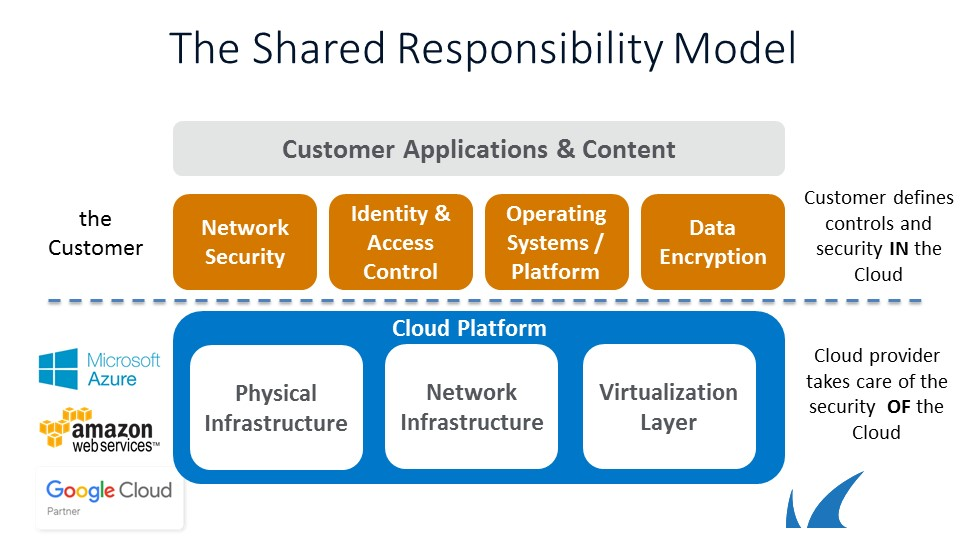
\includegraphics[width=0.5\textwidth]{figures/Shared_Responsibility_Model.jpg}}
	\caption{\label{fig:shared_responsibility_model} Shared responsibility model}%\cite{SecurityModel}
\end{figure}

	\item Data Privacy : Cloud computing involves the dispersal of data across servers located anywhere in
the world. Like globalization of networks. By crossing borders, involves considering
countries with restrictive privacy and protection laws . This is somewhat covered as
part of customer responsibility towards cloud security. For this corporations need to
understand what kind of data will they load into cloud and who will have access to
this data. [4]
Other aspect of data privacy is handling sensitive data. Yes one of the problems is
that this technology is light years ahead of the law and there are questions that need
to be answered. Who owns the data, consumer or the hosting cloud provider? Can
a cloud deny the consumer access to their own data or can it share this data with
marketing firms Obviously , the safest approach is data privacy is more a consumer
responsibility. Keep data under proper control and apply data encryption methods.
Regarding the question about laws, each company wants to protect their reputation.
To get more clients and maintain them, cloud providers would uphold your data
privacy. There are getting more managed and include all the necessary provisions
that one should take while setting up their data on cloud. [5] 

	\item ROI : ROI or Return of Investment is widely a measure of financial success and can be a measured in a variety of ways. If you move to public cloud, you generally decrease
investment but increase cost. With private cloud, it is vice-verse. But what matters
is value to business, customer value, seller value, market brand value, corporate value.
In case of cloud services, these relate to productivity, speed, size and quality. [6] 

	\item Integration Issues : Most enterprises would apply an incremental model of implementation. It is less risky than big-bang. This requires integration of services.The risk of not being able to integrate is critical. If you cannot build a system, you cannot use it. This also adds to the cost of including glue-software to connect various interfaces .It could involve rewrite of code or existing process models. Not to forget significant skills are required to assemble and customize multiple cloud services , requiring the applications to be loosely coupled, programmed to perform in an integration layer instead of underlying
infrastructure. 

\end{enumerate}



% needed in second column of first page if using \IEEEpubid
%\IEEEpubidadjcol


\section{Experiments }

Cloud computing is a change and if used in the right way, can be a great accelerator
of collaborated architecture. Cloud is an Internet phenomenon and trying to use
cloud the traditional enterprise way will not achieve real returns from the cloud. In
short Enterprises need to embrace new architecture.
One approach is using an incremental approach. This is less risky than big-bang
and also gives transition time to employees. This approach uses a hybrid cloud where
existing on-prem resources are connected to new resources on cloud. New external
cloud services can be incorporated in the in-house solutions, leading way to gradually
get rid of on-prem resources by their end of life.


\begin{figure}[h]
	\center{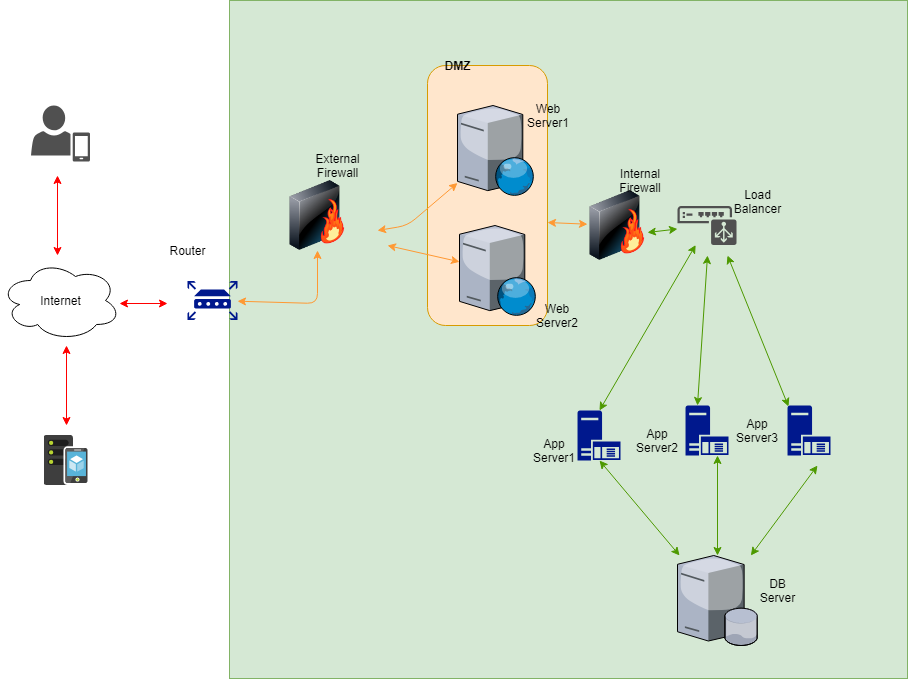
\includegraphics[width=0.5\textwidth]{figures/Current_State.png}}
	\caption{Sample on-premise architecture}%\cite{SecurityModel}
	\label{fig:Sample_on-premise_Architecture}
\end{figure}

Consider a general on-premise architecture as shown in \figref{Sample_on-premise_Architecture}. The different hybrid models among others that can be built are :
\begin{enumerate}
	\item Moving/extending storage and compute to cloud
	\item Moving backup/archive to cloud
	\item Moving business continuity or Disaster Recovery plan to cloud
\end{enumerate}

Depending on the flexibility of the existing on-premise architecture, storage and compute can be moved to cloud entirely , so that its basic advantages of scalability and reliability can be leveraged they can be used as an extension. In order to reap the benefits of cloud, moving components to cloud would be advisable rather than extending them. Moving on to the experiments of using the hybrid model, database from one of the cloud providers has been utilized to replicate the on-premise resource due to the limitations of creating a VPN or direct-connect as these seem to be costly options for an individual.For practical purposes, any corporation or industry will be already hosting a VPN or direct-connect to reduce latency.

\begin{enumerate}
	\item Azure Data Factory and SQL Database : As part of this experiment compute is moved to Azure Cloud by using Azure Data Factory. Azure Data Factory is a fully managed service provided by Microsoft that composes data storage, processing and movement services into streamlined, scalable, and reliable data production pipelines. To utilize compute in Azure Cloud a table sales\_records , is created in Azure SQL Database Cloud and an SSIS service in AzureDataFactory. Once SSIS service is deployed to Cloud it is scheduled to  run daily which computes sales data for every quarter and sales for every product based on region.
	\begin{figure}[!htb]
    \center{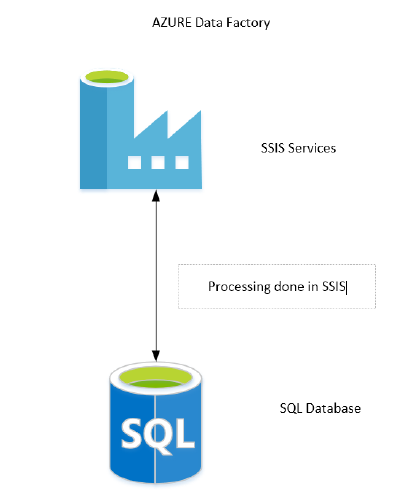
\includegraphics[width=0.3\textwidth]
    {figures/SSIS_ADF.png}}
    \caption{\label{fig:SSIS_ADF} SSIS Azure Data Factory}
	\end{figure}

	\begin{enumerate}
 		\item Create SQL Database. 
 		\begin{enumerate}
 			\item Login to Azure portal and click create SQL Database
			\item Create Cloud Computing database with a blank database
			\item Once DB is created, get the connection string for this database.
 		\end{enumerate}  
 		\item Create Azure Data Factory. 
 		\begin{enumerate}
 			\item Login to Azure portal and click Data + Analytics and click Data Factory
			\item Create unique name for SSIS Data Factory
			\item Click Author and Monitor.
			\item Click Configure SSIS Integration Runtime tile.
			\item On the SQL Settings page enter the configuration of the above SQL Database.
			\item Select Catalog Database Server Endpoint to host SSISDB.
 		\end{enumerate}  
	\end{enumerate}


	\item S3 –\(> Lambda \) –\(> DynamoDB \)  : As part of this experiment a csv file is uploaded to S3. AWS Lambda has a trigger whenever a new item is added to S3. Lambda function kicks in, it does its processing and uploads the data in csv file in S3 to DynamoDB. DynamoDB can process this data for end user or any analytic requirement. AWS Lambda is a server less architecture which utilizes resources required for processing the file in S3 to DynamoDB. Once the processing is complete the client is not charged unless the Lambda function is triggered again. To achieve this we followed the following steps: 
	
	\begin{figure}[h]
    \center{\includegraphics[width=0.6\textwidth]
    {figures/AWS_S3_Lambda_DynamoDB.png}}
    \caption{\label{fig:S3_DynamoDB} AWS Lambda S3 to DynamoDB}
	\end{figure}
%\begin{center}
%\includegraphics[scale=0.75]{figures/experiments/AWS_S3_Lambda_DynamoDB.png}
%\end{center}

\begin{enumerate}
 \item Create Policy in IAM. 
 \begin{enumerate}
 	\item Select S3, then select all actions and all resources
	\item Add additional permissions for DynamoDB, select all actions and all resources
	\item Add additional permissions for Cloudwatch, select all actions and all resources.
 \end{enumerate}  
 \item Create Role
 \begin{enumerate}
 	\item Attach the above policy to this role
\end{enumerate}
 \item Create Lambda Function
 \begin{enumerate} 
 	\item Create function, author from scratch
 	\item Give function name
 	\item Select runtime as Python 3.0
 	\item Choose existing role
 	\item Select role created above
 	\item Add trigger for S3, select bucket, event type (object created), prefix and filter if any.
 \end{enumerate}
\end{enumerate}



	\item AWS/Google Cloud –\(> Azure SQL Database \) : As part of this experiment, connectivity is tested between Amazon EC2 instance used for compute with SQL Server on Azure. 
	
	\begin{figure}[h]	
		\center{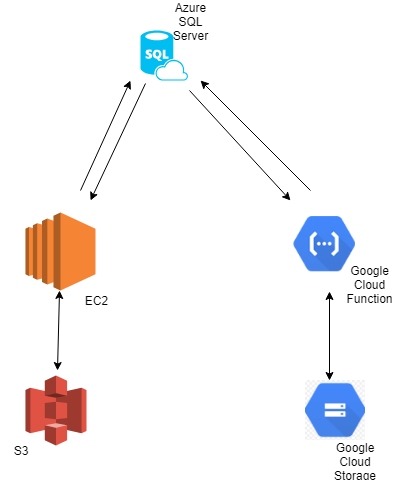
\includegraphics[width=0.30\textwidth]
		{figures/AWS_Google_Azure.png}}
    	\caption{\label{fig:AWS_Google_AzureDB} AWS to Azure and Google to Azure}
	\end{figure}
	
	\begin{enumerate} 
 		\item Connect to Azure SQL Server 
 		\begin{enumerate}
 			\item Create SQL Database. Steps remain same as discussed during Experiment (1)
 				
 		\end{enumerate}
 		
 		\item Connecting from AWS : Includes setting up EC2 instance with ability to connect to S3 and Azure.
 		\begin{enumerate}
 			\item Create user/IAM Roles to allow EC2 to connect to S3.Required role is "AmazonS3FullAccess" to the user.
 			\item Create EC2 instance with default configurations
 			\item login to EC2 instance with ec2-user and configure IAM role on EC2 to connect to S3 using aws configure. Use the access key ID and secret Access Key generated while creating IAM Roles. This is a one-time set up on EC2, even after a stop and restart the role is valid and available.
 			\item connection to s3 from EC2 can be now tested using aws s3 ls commands
 			\item Install sqlcmd on AWS EC2 and update firewall settings on Azure Sql server db to enable connections from EC2 instance
 			\item EC2 is ready to connect to SQl Server on Azure
 			
 		\end{enumerate}
 		\item Connecting from Google : Includes setting up python to connect to Azure from cloud shell. Google provides a shell environment for managing resources hosted on Google Cloud Platform. This allows us to test the connectivity without creating a Compute Engine.
 		\begin{enumerate}
 			\item Setting up Google cloud shell environment, requires installing python with some of its additional packages like pip,pyodbc and ODBC drivers including unixODBC and MSsql odbc 
 			\item Update firewall settings on Azure SQL Server DB to enable connections from Google shell.
 			\item connect using python pyodbc.connect  
 		\end{enumerate}
	 \end{enumerate}

 
\end{enumerate}
% An example of a floating figure using the graphicx package.
% Note that \label must occur AFTER (or within) \caption.
% For figures, \caption should occur after the \includegraphics.
% Note that IEEEtran v1.7 and later has special internal code that
% is designed to preserve the operation of \label within \caption
% even when the captionsoff option is in effect. However, because
% of issues like this, it may be the safest practice to put all your
% \label just after \caption rather than within \caption{}.
%
% Reminder: the "draftcls" or "draftclsnofoot", not "draft", class
% option should be used if it is desired that the figures are to be
% displayed while in draft mode.
%
%\begin{figure}[!t]
%\centering
%\includegraphics[width=2.5in]{myfigure}
% where an .eps filename suffix will be assumed under latex, 
% and a .pdf suffix will be assumed for pdflatex; or what has been declared
% via \DeclareGraphicsExtensions.
%\caption{Simulation results for the network.}
%\label{fig_sim}
%\end{figure}

% Note that the IEEE typically puts floats only at the top, even when this
% results in a large percentage of a column being occupied by floats.


% An example of a double column floating figure using two subfigures.
% (The subfig.sty package must be loaded for this to work.)
% The subfigure \label commands are set within each subfloat command,
% and the \label for the overall figure must come after \caption.
% \hfil is used as a separator to get equal spacing.
% Watch out that the combined width of all the subfigures on a 
% line do not exceed the text width or a line break will occur.
%
%\begin{figure*}[!t]
%\centering
%\subfloat[Case I]{\includegraphics[width=2.5in]{box}%
%\label{fig_first_case}}
%\hfil
%\subfloat[Case II]{\includegraphics[width=2.5in]{box}%
%\label{fig_second_case}}
%\caption{Simulation results for the network.}
%\label{fig_sim}
%\end{figure*}
%
% Note that often IEEE papers with subfigures do not employ subfigure
% captions (using the optional argument to \subfloat[]), but instead will
% reference/describe all of them (a), (b), etc., within the main caption.
% Be aware that for subfig.sty to generate the (a), (b), etc., subfigure
% labels, the optional argument to \subfloat must be present. If a
% subcaption is not desired, just leave its contents blank,
% e.g., \subfloat[].


% An example of a floating table. Note that, for IEEE style tables, the
% \caption command should come BEFORE the table and, given that table
% captions serve much like titles, are usually capitalized except for words
% such as a, an, and, as, at, but, by, for, in, nor, of, on, or, the, to
% and up, which are usually not capitalized unless they are the first or
% last word of the caption. Table text will default to \footnotesize as
% the IEEE normally uses this smaller font for tables.
% The \label must come after \caption as always.
%
%\begin{table}[!t]
%% increase table row spacing, adjust to taste
%\renewcommand{\arraystretch}{1.3}
% if using array.sty, it might be a good idea to tweak the value of
% \extrarowheight as needed to properly center the text within the cells
%\caption{An Example of a Table}
%\label{table_example}
%\centering
%% Some packages, such as MDW tools, offer better commands for making tables
%% than the plain LaTeX2e tabular which is used here.
%\begin{tabular}{|c||c|}
%\hline
%One & Two\\
%\hline
%Three & Four\\
%\hline
%\end{tabular}
%\end{table}


% Note that the IEEE does not put floats in the very first column
% - or typically anywhere on the first page for that matter. Also,
% in-text middle ("here") positioning is typically not used, but it
% is allowed and encouraged for Computer Society conferences (but
% not Computer Society journals). Most IEEE journals/conferences use
% top floats exclusively. 
% Note that, LaTeX2e, unlike IEEE journals/conferences, places
% footnotes above bottom floats. This can be corrected via the
% \fnbelowfloat command of the stfloats package.




\section{Conclusions and Future Work}
In this paper we have tried different connectivity options to connect 1 cloud environment to a database in another cloud. We considered simple approaches , single connect options with comparatively less amount of data. Same options can be used in a scaled resource on cloud without much ado.

While the three cloud environments considered have almost similar type of features or resources available, in order to reap the benefits of cloud, a use-cased based architecture should be considered. Working on cloud does require added skills as segregation of duties is lessened. Needless to say, cloud does not eliminate the need of your platform team. Security of cloud is still a shared responsibility. 

In future work  we will experiment on creating VPC tunnel between the different cloud environments. This will be close to real application of a hybrid cloud. Hybrid cloud allows collaboration of multiple cloud services as per requirement . Another feature that we will like to study is the use of multi-cloud structure for backup and recovery.


% if have a single appendix:
%\appendix[Proof of the Zonklar Equations]
% or
%\appendix  % for no appendix heading
% do not use \section anymore after \appendix, only \section*
% is possibly needed

% use appendices with more than one appendix
% then use \section to start each appendix
% you must declare a \section before using any
% \subsection or using \label (\appendices by itself
% starts a section numbered zero.)
%


\appendices
\section{Cloud Resources}

\subsection{S3}

S3 - stands for Simple Storage Service. This service could be utilized to collect, store and analyze huge amounts of data. Data stored in S3 could be retrieved from anywhere. It provides comprehensive security and compliance capabilities. S3 is designed to deliver 99.999999999\% durability. Some of the other features/advantages are :

\begin{enumerate}
	\item Unmatched Durability, Availability \& Scability
	\item Most comprehensive security \& compliance capabilities
	\item Query in place
	\item Flexible management
	\item Most supported by partners, vendors \& AWS serices
	\item Easy, Flexible data transfer
\end{enumerate}

\subsection{Google Cloud Storage}

Google Cloud Storage is a RESTful online file storage web service for storing and accessing data on Google Cloud Platform infrastructure. It is comparable to Amazon S3 . Contrary to Google Drive, this is more suitable for enterprises.Some of the other features/advantages are [7] :

\begin{enumerate}
	\item designed for 99.999999999\% durability. It stores data redundantly with automatic checksums to ensure data integrity.
	\item highly scalable . Objects larger than 5MB should be uploaded with multipart or resumable uploading.Google Storage provides a resumable data transfer feature that allows user to resume upload operations after a communication failure has interrupted the flow of data.
	\item Google Storage is interoperable with other cloud storage tools and libraries
	\item  Upload operations to Google Storage are atomic , providing strong read-after-write consistency for all upload operations
\end{enumerate}

\subsection{Dynamo DB} 
Amazon DynamoDB is a non-relational database that delivers reliable performance at any scale. Some of the other features/advantages are :

\begin{enumerate}
	\item Performance at scale
	\item Fully managed
	\item Enterprise-ready
\end{enumerate}

\subsection{Elastic Compute Cloud (EC2)} 
Amazon Elastic Comput Cloud is a web service that provides secure, re sizable compute capacity in the cloud. EC2 has changed the economics of computing by allowing companies to pay only for the capacity that is being utilized.Some of the other features/advantages are :

\begin{enumerate}
	\item Elastic web-scale computing
	\item Completely controlled
	\item Flexible cloud hosting services
	\item Integrated
	\item Reliable
	\item Secure
	\item Inexpensive
	\item Easy to start
\end{enumerate}

\subsection{AWS Lambda} 
AWS Lambda can run code without provisioning or managing servers. We have to pay only for the compute time consumed.Some of the other features/advantages are :

\begin{enumerate}
	\item No servers to manage
	\item Continuous scaling
	\item Subsecond metering
\end{enumerate}

\subsection{Azure SQL Database}
This is a relational database-as-a-service (DBaaS) with the latest version of Microsoft SQL Server Database Engine. It is high performance, reliable and secure database on which data-driven applications and websites can be built in the programming language of choice without needing to manage infrastructure. Some of the other features/advantages are :

\begin{enumerate}
	\item Fully managed
	\item Advanced security
	\item Built-in intelligence
\end{enumerate}

% you can choose not to have a title for an appendix
% if you want by leaving the argument blank
%\section{Additional Notes}
% Appendix two text goes here.


% use section* for acknowledgment
\section*{Acknowledgment}


The authors would like to thank Dr Sohail Rafiqi for giving us the opportunity to work on this paper and showing us a liberal approach towards cloud . There is no right answer and there is no right model. 

% Can use something like this to put references on a page
% by themselves when using endfloat and the captionsoff option.
\ifCLASSOPTIONcaptionsoff
  \newpage
\fi



% trigger a \newpage just before the given reference
% number - used to balance the columns on the last page
% adjust value as needed - may need to be readjusted if
% the document is modified later
%\IEEEtriggeratref{}
% The "triggered" command can be changed if desired:
%\IEEEtriggercmd{\enlargethispage{-5in}}

% references section

\section{REFERENCES}
%\begin{frame}[fragile]
%\frametitle{External Link Example}

\begin{verbatim}
[1] Online {https://www.marutitech.com/5-reasons-why-cloud-can-transform-your-business}
[2] Online {https://www.salesforce.com/uk/blog/2015/11/why-move-to-the-cloud-10-benefits-of-cloud-computing.html}
[3] Online {https://insights.sei.cmu.edu/sei_blog/2018/03/12-risks-threats-vulnerabilities-in-moving-to-the-cloud.html}
[4] Online {https://legal.thomsonreuters.com/en/insights/articles/understanding-data-privacy-and-cloud-computing}
[5] Online {https://www.privacyrights.org/blog/privacy-implications-cloud-computing}
[6] Online {http://www.opengroup.org/cloud/cloud_for_business/p6.htm}
[7] Online {https://cloud.google.com/storage/features/}
\end{verbatim}



%\\[15pt]
%\url{https://insights.sei.cmu.edu/sei_blog/2018/03/12-risks-threats-vulnerabilities-in-moving-to-the-cloud.html}
%\end{frame}


% can use a bibliography generated by BibTeX as a .bbl file
% BibTeX documentation can be easily obtained at:
% http://mirror.ctan.org/biblio/bibtex/contrib/doc/
% The IEEEtran BibTeX style support page is at:
% http://www.michaelshell.org/tex/ieeetran/bibtex/
%\bibliographystyle{IEEEtran}
% argument is your BibTeX string definitions and bibliography database(s)
%\bibliography{IEEEabrv,../bib/paper}
%
% <OR> manually copy in the resultant .bbl file
% set second argument of \begin to the number of references
% (used to reserve space for the reference number labels box)








\begin{thebibliography}{1}

\bibitem{IEEEhowto:kopka}



\end{thebibliography}

% biography section
% 
% If you have an EPS/PDF photo (graphicx package needed) extra braces are
% needed around the contents of the optional argument to biography to prevent
% the LaTeX parser from getting confused when it sees the complicated
% \includegraphics command within an optional argument. (You could create
% your own custom macro containing the \includegraphics command to make things
% simpler here.)
%\begin{IEEEbiography}[{\includegraphics[width=1in,height=1.25in,clip,keepaspectratio]{mshell}}]{Michael Shell}
% or if you just want to reserve a space for a photo:

%\begin{IEEEbiography}{Mahesh Kuklani}
%Biography text here.
%\end{IEEEbiography}

% if you will not have a photo at all:
\begin{IEEEbiographynophoto}{Mahesh Kuklani}
Mahesh Kuklani is currently working towards his Master's degree in Data Science at Southern Methodist University, Dallas , TX.
\end{IEEEbiographynophoto}

% insert where needed to balance the two columns on the last page with
% biographies
%\newpage

\begin{IEEEbiographynophoto}{Tanvi Arora}
Tanvi Arora received the bachelor's degree in Computer Science Engineering from University of Rajasthan, India . She is currently working towards her Master's degree in Data Science at Southern Methodist University, Dallas , Texas.She works full time as a Senior Software Developer in USA and has about 11 years of work experience in this field .
\end{IEEEbiographynophoto}

% You can push biographies down or up by placing
% a \vfill before or after them. The appropriate
% use of \vfill depends on what kind of text is
% on the last page and whether or not the columns
% are being equalized.

%\vfill

% Can be used to pull up biographies so that the bottom of the last one
% is flush with the other column.
%\enlargethispage{-5in}



% that's all folks
\end{document}


